\documentclass[tcc,capa]{texufpel}

\usepackage[latin1]{inputenc} % acentuacao
\usepackage{graphicx} % para inserir figuras

\unidade{Centro de Desenvolvimento Tecnol�gico}
\curso{Engenharia de Computa��o}
\nomecurso{Bacharelado em Engenharia de Computa��o}
\titulocurso{Bacharel em Engenharia de Computa��o}

\title{Uma plataforma para consci�ncia de contexto utilizando Computa��o em Nuvem}

\author{Goebel}{Guilherme Davesac}
\advisor[Prof.~Dr.]{Soares}{Rafael Iankowski}
\coadvisor[Prof.~Dr.]{Yamin}{Adenauer Corr�a}


\keyword{Nuvem}
\keyword{FIWARE}
\keyword{CoT}
\keyword{IoT}

\begin{document}

%\renewcommand{\advisorname}{Orientadora}           %descomente caso tenhas orientadora
%\renewcommand{\coadvisorname}{Coorientadora}      %descomente caso tenhas coorientadora

\maketitle 

\sloppy

\fichacatalografica

\folhadeaprovacao

%Opcional
%\begin{dedicatoria}
%  Dedico\ldots bla blabla blablabla bla. Bla blabla blablabla bla.\\
%  Bla blabla blablabla bla. Bla blabla blablabla bla.
%\end{dedicatoria}

%Opcional
%\begin{agradecimentos}
%  Bla blabla blablabla bla.  Bla blabla blablabla bla.  Bla blabla blablabla
%  bla.  Bla blabla blablabla bla.  Bla blabla blablabla bla.  Bla blabla
%  blablabla bla.  Bla blabla blablabla bla.  Bla blabla blablabla bla.  Bla
%  blabla blablabla bla.  Bla blabla blablabla bla.  Bla blabla blablabla bla.
%  Bla blabla blablabla bla.  Bla blabla blablabla bla.  Bla blabla blablabla
%  bla.  Bla blabla blablabla bla.  Bla blabla blablabla bla.  Bla blabla
%  blablabla bla.  Bla blabla blablabla bla.  Bla blabla blablabla bla.  Bla
%  blabla blablabla bla.  Bla blabla blablabla bla.
%\end{agradecimentos}

%Opcional
%\begin{epigrafe}
%  Bla blabla blablabla bla.\\
%  Bla blabla blablabla bla.\\
%  Bla blabla blablabla bla.\\
%  Bla blabla blablabla bla.\\
%  Bla blabla blablabla bla.\\
%  {\sc --- Fulano de Tal}
%\end{epigrafe}

%Resumo em Portugues (no maximo 500 palavras)
\begin{abstract}
  Resumo em portugu�s sobre o trabalho de conclus�o de curso: 
\end{abstract}

\begin{englishabstract}%
  {Titulo do Trabalho em Ingles}%
  {Cloud, Fiware, CoT, IoT}
  
  Resumo em Ingl�s.
\end{englishabstract}

%Lista de Figuras
\listoffigures

%Lista de Tabelas
\listoftables

%lista de abreviaturas e siglas
\begin{listofabbrv}{SPMD}
        \item[CoT] Cloud of Things
        \item[IoT] Internet of Things
        \item[TCC] Trabalho de Conclus�o de Curso
        \item[UbiComp] Computa��o Ub�qua
        \item[ABNT] Associa��o Brasileira de Normas T�cnicas
\end{listofabbrv}

%Sumario
\tableofcontents

\chapter{Introdu��o}

\section{Motiva��o e Objetivos}

  Bla blabla blablabla bla.  Bla blabla blablabla bla.  Bla blabla blablabla
  bla.  Bla blabla blablabla bla.  Bla blabla blablabla bla.  Bla blabla
  blablabla bla.  Bla blabla blablabla bla.  Bla blabla blablabla bla.  Bla
  blabla blablabla bla.  Bla blabla blablabla bla.  Bla blabla blablabla bla.
  Bla blabla blablabla bla.  Bla blabla blablabla bla.  Bla blabla blablabla
  bla.  Bla blabla blablabla bla.  Bla blabla blablabla bla.  Bla blabla
  blablabla bla.  Bla blabla blablabla bla.  Bla blabla blablabla bla.  Bla
  blabla blablabla bla.  Bla blabla blablabla bla.

  Bla blabla blablabla bla.  Bla blabla blablabla bla.  Bla blabla blablabla
  bla.  Bla blabla blablabla bla.  Bla blabla blablabla bla.  Bla blabla
  blablabla bla.  Bla blabla blablabla bla.  Bla blabla blablabla bla.  Bla
  blabla blablabla bla.  Bla blabla blablabla bla.  Bla blabla blablabla bla.
  Bla blabla blablabla bla.  Bla blabla blablabla bla.  Bla blabla blablabla
  bla.  Bla blabla blablabla bla.  Bla blabla blablabla bla.  Bla blabla
  blablabla bla.  Bla blabla blablabla bla.  Bla blabla blablabla bla.  Bla
  blabla blablabla bla.  Bla blabla blablabla bla~\citet{Moore:1979:MAI,Aguiar:2005}.

  Bla blabla blablabla bla.  Bla blabla blablabla bla.  Bla blabla blablabla
  bla.  Bla blabla blablabla bla.  Bla blabla blablabla bla.  Bla blabla
  blablabla bla.  Bla blabla blablabla bla.  Bla blabla blablabla bla.  Bla
  blabla blablabla bla.  Bla blabla blablabla bla.  Bla blabla blablabla bla.
  Bla blabla blablabla bla.  Bla blabla blablabla bla.  Bla blabla blablabla
  bla.  Bla blabla blablabla bla.  Bla blabla blablabla bla.  Bla blabla
  blablabla bla.  Bla blabla blablabla bla.  Bla blabla blablabla bla.  Bla
  blabla blablabla bla.  Bla blabla blablabla bla~\cite{vonNeumann:1966:TSR}.

\section{Estrutura do Texto}

  Bla blabla blablabla bla.  Bla blabla blablabla bla.  Bla blabla blablabla
  bla.  Bla blabla blablabla bla.  Bla blabla blablabla bla.  Bla blabla
  blablabla bla.  Bla blabla blablabla bla.  Bla blabla blablabla bla.  Bla
  blabla blablabla bla.  Bla blabla blablabla bla.  Bla blabla blablabla bla.
  Bla blabla blablabla bla.  Bla blabla blablabla bla.  Bla blabla blablabla
  bla.  Bla blabla blablabla bla.  Bla blabla blablabla bla.  Bla blabla
  blablabla bla.  Bla blabla blablabla bla.  Bla blabla blablabla bla.  Bla
  blabla blablabla bla.  Bla blabla blablabla bla~\ref{tabela}.

\begin{table}
\begin{center}
\caption{Nome da Tabela}\label{tabela}
\begin{tabular}{p{4cm}p{5cm}p{6cm}}
\hline
Blabla & Blabla & Blablabla\\
\hline
{\small Bla} & {\small Blabla} & {\small\em Bla blabla blablabla blabla
  blablabla blabla blablabla.}\\
{\small Bla} & {\small Blabla} & {\small\em Bla blabla blablabla blabla
  blablabla blabla blablabla.}\\
{\small Bla} & {\small Blabla} & {\small\em Bla blabla blablabla blabla
  blablabla blabla blablabla.}\\
{\small Bla} & {\small Blabla} & {\small\em Bla blabla blablabla blabla
  blablabla blabla blablabla.}\\
{\small Bla} & {\small Blabla} & {\small\em Bla blabla blablabla blabla
  blablabla blabla blablabla.}\\
{\small Bla} & {\small Blabla} & {\small\em Bla blabla blablabla blabla
  blablabla blabla blablabla.}\\
\hline
\end{tabular}
\end{center}
\end{table}

\subsection{Uma subse��o}

  Bla blabla blablabla bla.  Bla blabla blablabla bla.  Bla blabla blablabla
  bla.  Bla blabla blablabla bla.  Bla blabla blablabla bla.  Bla blabla
  blablabla bla.  Bla blabla blablabla bla.  Bla blabla blablabla bla.  Bla
  blabla blablabla bla.  Bla blabla blablabla bla.  Bla blabla blablabla bla.
  Bla blabla blablabla bla.  Bla blabla blablabla bla.  Bla blabla blablabla
  bla.  Bla blabla blablabla bla.  Bla blabla blablabla bla.  Bla blabla
  blablabla bla.  Bla blabla blablabla bla.  Bla blabla blablabla bla.  Bla
  blabla blablabla bla.  Bla blabla blablabla bla.

\chapter{Internet of Things e Cloud of Things: Evolu��o }

  Bla blabla blablabla bla.  Bla blabla blablabla bla.  Bla blabla
  blablabla bla.  Bla blabla blablabla bla.  Bla blabla blablabla bla.
  Bla blabla blablabla bla.  Bla blabla blablabla bla.  Bla blabla
  blablabla bla.  Bla blabla blablabla bla.  Bla blabla blablabla bla.
  Bla blabla blablabla bla.  Bla blabla blablabla bla.  Bla blabla
  blablabla bla.  Bla blabla blablabla bla.  Bla blabla blablabla bla.
  Bla blabla blablabla bla.  Bla blabla blablabla bla.  Bla blabla
  blablabla bla.  Bla blabla blablabla bla.  Bla blabla blablabla bla.
  Bla blabla blablabla bla~\ref{tabela2}.
\section{Internet of Things: }
bla bla bla

\section{Cloud of Things: }

\begin{table}
\begin{center}
\caption{Nome da Tabela}\label{tabela2}
\begin{tabular}{p{4cm}p{5cm}p{6cm}}
\hline
Blabla & Blabla & Blablabla\\
\hline
{\small Bla} & {\small Blabla} & {\small\em Bla blabla blablabla blabla
  blablabla blabla blablabla.}\\
{\small Bla} & {\small Blabla} & {\small\em Bla blabla blablabla blabla
  blablabla blabla blablabla.}\\
{\small Bla} & {\small Blabla} & {\small\em Bla blabla blablabla blabla
  blablabla blabla blablabla.}\\
{\small Bla} & {\small Blabla} & {\small\em Bla blabla blablabla blabla
  blablabla blabla blablabla.}\\
{\small Bla} & {\small Blabla} & {\small\em Bla blabla blablabla blabla
  blablabla blabla blablabla.}\\
{\small Bla} & {\small Blabla} & {\small\em Bla blabla blablabla blabla
  blablabla blabla blablabla. Conforme a figura~\ref{figura}}\\
\hline
\end{tabular}
\end{center}
\end{table}

\begin{figure}[htbp]
  \centering 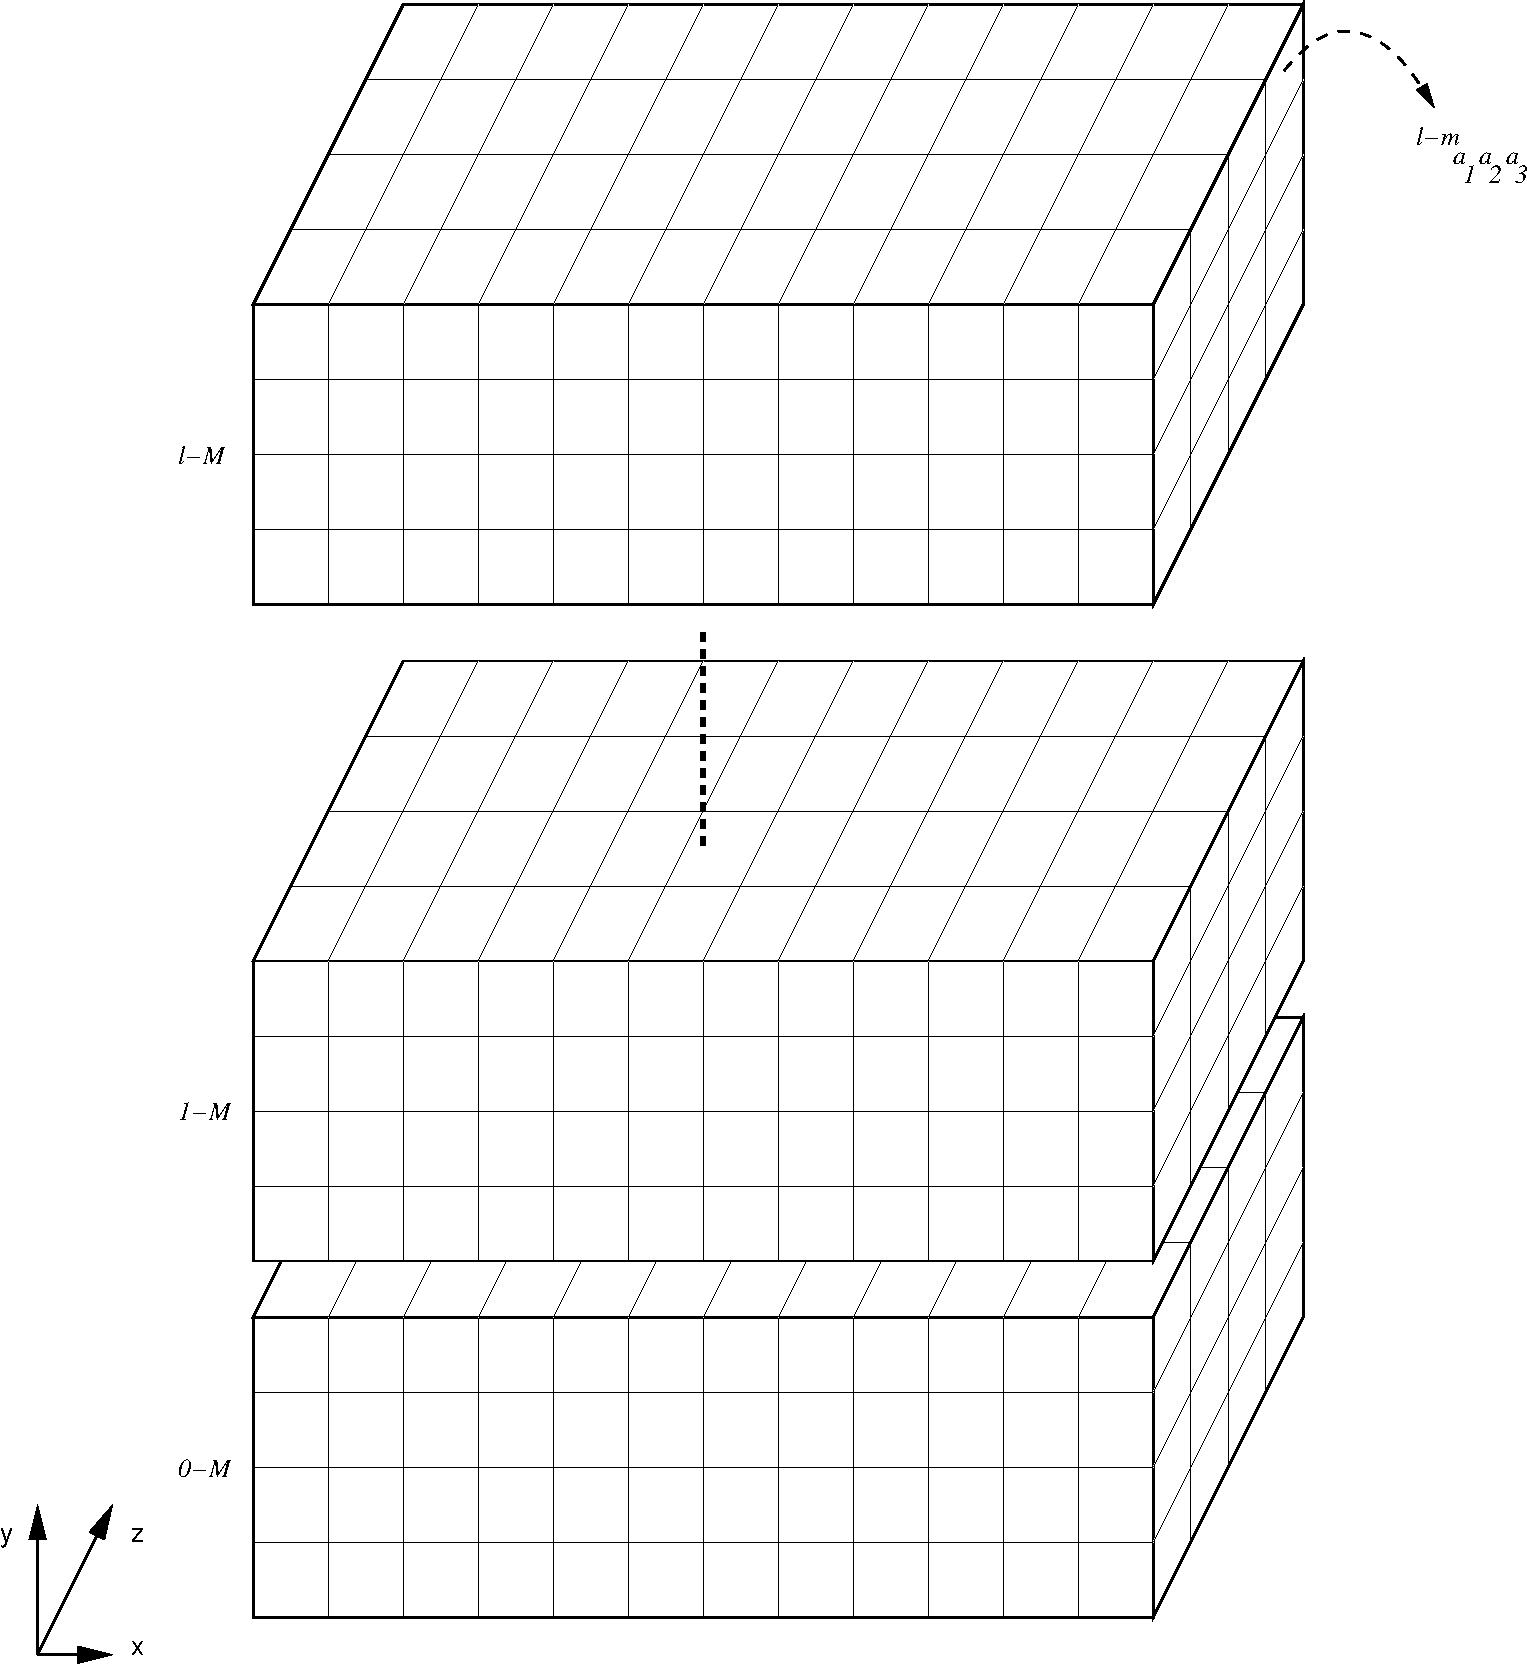
\includegraphics[scale=.4]{figura}
\caption{Nome da figura} 
\label{figura}
\end{figure}


\chapter{Trabalhos relacionados: }

  Bla blabla blablabla bla.  Bla blabla blablabla bla.  Bla blabla blablabla
  bla.  Bla blabla blablabla bla.  Bla blabla blablabla bla.  Bla blabla
  blablabla bla.  Bla blabla blablabla bla.  Bla blabla blablabla bla.  Bla
  blabla blablabla bla.  Bla blabla blablabla bla.  Bla blabla blablabla bla.
  Bla blabla blablabla bla.  Bla blabla blablabla bla.  Bla blabla blablabla
  bla.  Bla blabla blablabla bla.  Bla blabla blablabla bla.  Bla blabla
  blablabla bla.  Bla blabla blablabla bla.  Bla blabla blablabla bla.  Bla
  blabla blablabla bla.  Bla blabla blablabla bla.

  Bla blabla blablabla bla.  Bla blabla blablabla bla.  Bla blabla blablabla
  bla.  Bla blabla blablabla bla.  Bla blabla blablabla bla.  Bla blabla
  blablabla bla.  Bla blabla blablabla bla.  Bla blabla blablabla bla.  Bla
  blabla blablabla bla.  Bla blabla blablabla bla.  Bla blabla blablabla bla.
  Bla blabla blablabla bla.  Bla blabla blablabla bla.  Bla blabla blablabla
  bla.  Bla blabla blablabla bla.  Bla blabla blablabla bla.  Bla blabla
  blablabla bla.  Bla blabla blablabla bla.  Bla blabla blablabla bla.  Bla
  blabla blablabla bla.  Bla blabla blablabla bla.
\section{T�tulo 1}
\section{T�tulo N}

\chapter{EXEHDA ? }

bla bla
  
\chapter{FIWARE: Um estudo sobre a tecnologia }

\chapter{Conclus�o}

% Bibliografia
% http://liinwww.ira.uka.de/bibliography/index.html
% um site que cataloga no formato bibtex a bibliografia em computacao
%\bibliography{nomedoarquivo.bib} (sem extensao)
%\bibliographystyle{formato.bst} (sem extensao)

\bibliography{bibliografia}
\bibliographystyle{abnt}

% Anexos (Opcional)
\annex 
\chapter{Um Anexo}

  Bla blabla blablabla bla.  Bla blabla blablabla bla.  Bla blabla blablabla
  bla.  Bla blabla blablabla bla.  Bla blabla blablabla bla.  Bla blabla
  blablabla bla.  Bla blabla blablabla bla.  Bla blabla blablabla bla.  Bla
  blabla blablabla bla.  Bla blabla blablabla bla.  Bla blabla blablabla bla.
  Bla blabla blablabla bla.  Bla blabla blablabla bla.  Bla blabla blablabla
  bla.  Bla blabla blablabla bla.  Bla blabla blablabla bla.  Bla blabla
  blablabla bla.  Bla blabla blablabla bla.  Bla blabla blablabla bla.  Bla
  blabla blablabla bla.  Bla blabla blablabla bla.

  Bla blabla blablabla bla.  Bla blabla blablabla bla.  Bla blabla blablabla
  bla.  Bla blabla blablabla bla.  Bla blabla blablabla bla.  Bla blabla
  blablabla bla.  Bla blabla blablabla bla.  Bla blabla blablabla bla.  Bla
  blabla blablabla bla.  Bla blabla blablabla bla.  Bla blabla blablabla bla.
  Bla blabla blablabla bla.  Bla blabla blablabla bla.  Bla blabla blablabla
  bla.  Bla blabla blablabla bla.  Bla blabla blablabla bla.  Bla blabla
  blablabla bla.  Bla blabla blablabla bla.  Bla blabla blablabla bla.  Bla
  blabla blablabla bla.  Bla blabla blablabla bla.

\chapter{Outro Anexo}

  Bla blabla blablabla bla.  Bla blabla blablabla bla.  Bla blabla blablabla
  bla.  Bla blabla blablabla bla.  Bla blabla blablabla bla.  Bla blabla
  blablabla bla.  Bla blabla blablabla bla.  Bla blabla blablabla bla.  Bla
  blabla blablabla bla.  Bla blabla blablabla bla.  Bla blabla blablabla bla.
  Bla blabla blablabla bla.  Bla blabla blablabla bla.  Bla blabla blablabla
  bla.  Bla blabla blablabla bla.  Bla blabla blablabla bla.  Bla blabla
  blablabla bla.  Bla blabla blablabla bla.  Bla blabla blablabla bla.  Bla
  blabla blablabla bla.  Bla blabla blablabla bla.

  Bla blabla blablabla bla.  Bla blabla blablabla bla.  Bla blabla blablabla
  bla.  Bla blabla blablabla bla.  Bla blabla blablabla bla.  Bla blabla
  blablabla bla.  Bla blabla blablabla bla.  Bla blabla blablabla bla.  Bla
  blabla blablabla bla.  Bla blabla blablabla bla.  Bla blabla blablabla bla.
  Bla blabla blablabla bla.  Bla blabla blablabla bla.  Bla blabla blablabla
  bla.  Bla blabla blablabla bla.  Bla blabla blablabla bla.  Bla blabla
  blablabla bla.  Bla blabla blablabla bla.  Bla blabla blablabla bla.  Bla
  blabla blablabla bla.  Bla blabla blablabla bla.

%Faz a capa do CDROM
\makecover

\end{document}

